\documentclass{article}
\usepackage{amsmath}
\usepackage{amsthm}
\usepackage{graphicx}
\usepackage{tikz}
\usepackage{pgfplots}
\usepackage{booktabs}
\usepackage{enumitem}
\usepackage[margin=1in]{geometry}
\usepackage{titlesec}
\titleformat{\section}[block]{\normalfont\large\bfseries\centering}{\thesection}{1em}{}
\titleformat{\subsection}[block]{\normalfont\bfseries\centering}{\thesubsection}{1em}{}
\theoremstyle{definition}
\newtheorem{definition}{Definition}
\newtheorem{example}{Example}
\title{Study Notes: Chapter 3 - Describing Bivariate Data}
\author{Antony Lotter}
\date{\today}
\begin{document}
	\maketitle
	\section{Introduction to Chapter 3}
	This chapter explores bivariate data—measurements of two variables on a single experimental unit. It covers methods to display and describe relationships between variables, whether categorical or quantitative. Focus is on sections 3.1 (categorical data) and 3.2 (quantitative data), emphasizing graphical and numerical summaries to reveal patterns, such as associations or trends.
	Detailed Explanation: Bivariate analysis goes beyond univariate by examining how variables interact. For example, does household size affect grocery spending? Graphs and statistics help identify dependencies, strengths, and forms of relationships.
	\section*{3.1 Describing Bivariate Categorical Data}
	\subsection{Key Concepts}
	When at least one variable is qualitative (categorical), use pie charts, bar charts (side-by-side or stacked), or line charts to display data. These reveal comparisons across categories or groups.
	\begin{definition}[Contingency Table]
		A table showing frequencies (counts) or relative frequencies for combinations of two categorical variables.
	\end{definition}
	\begin{definition}[Conditional Distribution]
		Proportions within one category given a condition on the other (e.g., proportions by rank given college type).
	\end{definition}
	Detailed Explanation: For bivariate categorical data, summarize using frequencies in a contingency table. Visualize with:
	
	Side-by-side bar charts: Compare groups within categories.
	Stacked bar charts: Show composition within totals.
	Side-by-side pie charts: Display proportions per group.
	
	Relative frequencies (proportions) aid comparison when group sizes differ.
	\subsection{Examples}
	\begin{example}[Salaries of Professors]
		Data on 400 professors: rank (Full, Associate, Assistant) and college type (Public, Private). Average salaries (thousands \$):
	\end{example}	
		\begin{table}[ht]
			\centering
			\begin{tabular}{lccc}
				\toprule
				& Full Professor & Associate Professor & Assistant Professor \\
				\midrule
				Public & 108.9 & 80.9 & 69.2 \\
				Private & 127.8 & 84.5 & 69.7 \\
				\bottomrule
			\end{tabular}
			\caption{Salaries of Professors by Rank and Type of College}
		\end{table}
		Side-by-side bar chart (Figure 3.1) shows higher salaries for full professors in private colleges, with smaller differences at lower ranks.
		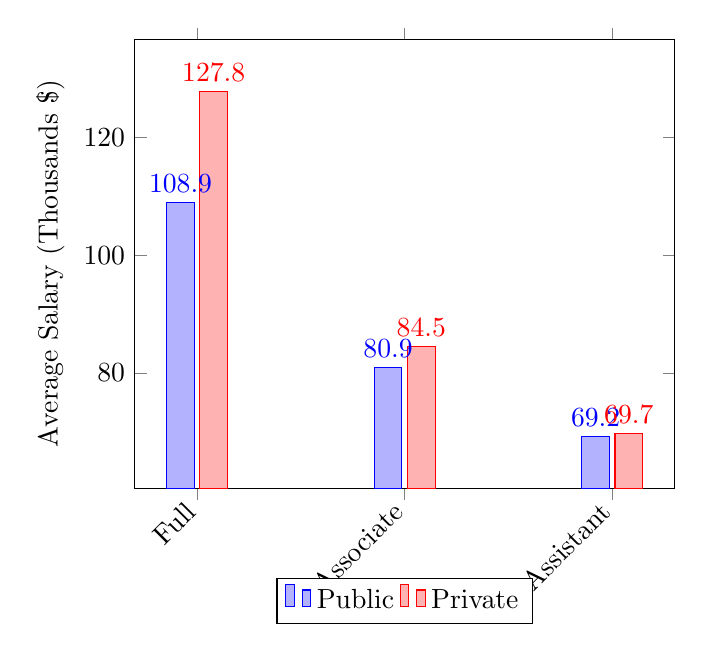
\begin{tikzpicture}
			\begin{axis}
				[
				ybar,
				enlargelimits=0.15,
				ylabel={Average Salary (Thousands \$)},
				symbolic x coords={Full, Associate, Assistant},
				xtick=data,
				nodes near coords,
				nodes near coords align={vertical},
				x tick label style={rotate=45,anchor=east},
				legend style={at={(0.5,-0.2)}, anchor=north, legend columns=-1},
				]
				\addplot coordinates {(Full,108.9) (Associate,80.9) (Assistant,69.2)};
				\addlegendentry{Public}
				\addplot coordinates {(Full,127.8) (Associate,84.5) (Assistant,69.7)};
				\addlegendentry{Private}
			\end{axis}
		\end{tikzpicture}
	\begin{example}[Number of Professors by Rank and Type]
		Counts for same categories:
		\begin{table}[ht]
			\centering
			\begin{tabular}{lcccc}
				\toprule
				& Full Professor & Associate Professor & Assistant Professor & Total \\
				\midrule
				Public & 24 & 57 & 69 & 150 \\
				Private & 60 & 78 & 112 & 250 \\
				\bottomrule
			\end{tabular}
			\caption{Number of Professors by Rank and Type of College}
		\end{table}
		Side-by-side pie charts or stacked bar chart show private colleges have more full professors proportionally.
		Stacked bar chart visualization:
		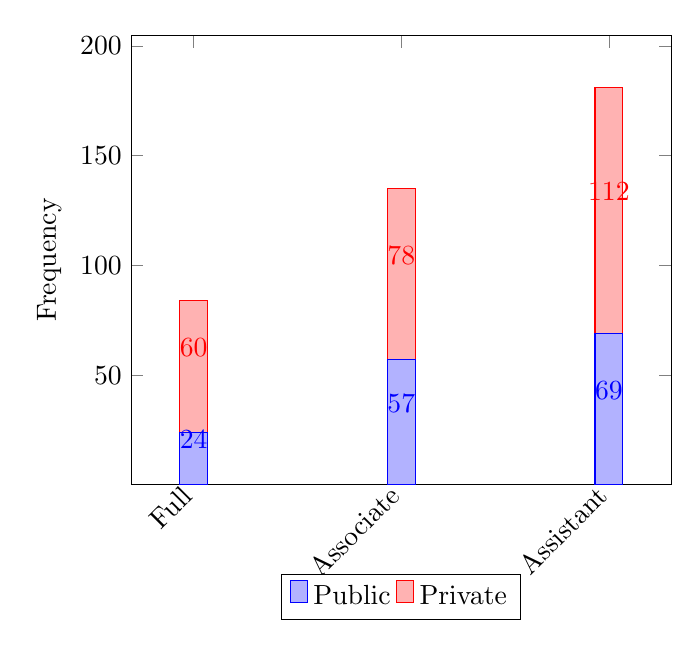
\begin{tikzpicture}
			\begin{axis}
				[
				ybar stacked,
				enlargelimits=0.15,
				ylabel={Frequency},
				symbolic x coords={Full, Associate, Assistant},
				xtick=data,
				nodes near coords,
				nodes near coords align={vertical},
				x tick label style={rotate=45,anchor=east},
				legend style={at={(0.5,-0.2)}, anchor=north, legend columns=-1},
				]
				\addplot coordinates {(Full,24) (Associate,57) (Assistant,69)};
				\addlegendentry{Public}
				\addplot coordinates {(Full,60) (Associate,78) (Assistant,112)};
				\addlegendentry{Private}
			\end{axis}
		\end{tikzpicture}
		Conditional distributions (proportions by type):
		\begin{table}[ht]
			\centering
			\begin{tabular}{lcccc}
				\toprule
				& Full Professor & Associate Professor & Assistant Professor & Total \\
				\midrule
				Public & 0.16 & 0.38 & 0.46 & 1.00 \\
				Private & 0.24 & 0.31 & 0.45 & 1.00 \\
				\bottomrule
			\end{tabular}
			\caption{Proportions of Professors by Rank for Public and Private Colleges (Table 3.3)}
		\end{table}
		Public colleges have fewer full professors (16% vs. 24%) and more associates.
	\end{example}
	\section{3.2 Describing Bivariate Quantitative Data}
	\subsection{Scatterplots}
	Plot quantitative variables on (x, y) axes to visualize patterns.
	Detailed Explanation: Scatterplots reveal trends (linear, curved, none), strength (tight vs. loose clustering), direction (positive/negative), outliers, or clusters. Independent variable (x) on horizontal, dependent (y) on vertical if applicable.
	\begin{example}[Household Size and Grocery Spending]
		Data: x (members), y (spending \$):
		\begin{table}[ht]
			\centering
			\begin{tabular}{ccccccc}
				\toprule
				x & 2 & 3 & 3 & 4 & 1 & 5 \\
				y & 384 & 421 & 465 & 546 & 207 & 621 \\
				\bottomrule
			\end{tabular}
			\caption{Household Members and Weekly Grocery Spending}
		\end{table}
		Scatterplot (Figure 3.4) shows positive linear trend; outlier at (2, 556) deviates.
		\begin{tikzpicture}
			\begin{axis}[
				xlabel={x (Members)},
				ylabel={y (Spending \$)},
				xmin=0, xmax=6,
				ymin=0, ymax=700,
				]
				\addplot[only marks] coordinates {(2,384) (3,421) (3,465) (4,546) (1,207) (5,621)};
				\addplot[only marks, mark=x] coordinates {(2,556)};
			\end{axis}
		\end{tikzpicture}
	\end{example}
	\begin{example}[Wine Price and Demand]
		Data: price (\$12-16), cases sold (per 10,000 pop.):
		Scatterplot (Figure 3.5) shows curved pattern: demand decreases then increases.
		\begin{tikzpicture}
			\begin{axis}[
				xlabel={Price (\$)},
				ylabel={Cases Sold},
				xmin=11, xmax=17,
				ymin=15, ymax=26,
				]
				\addplot[only marks] coordinates {(12,23) (12,21) (13,19) (13,18) (14,15) (14,17) (15,19) (15,20) (16,25) (16,24)};
			\end{axis}
		\end{tikzpicture}
	\end{example}
	\subsection{The Correlation Coefficient}
	Measures strength and direction of linear relationship.
	\begin{definition}[Sample Correlation Coefficient]
		$   r = \frac{s_{xy}}{s_x s_y}   $
		where $  s_{xy} = \frac{\sum (x_i - \bar{x})(y_i - \bar{y})}{n-1}  $ (covariance).
	\end{definition}
	Detailed Explanation: r ranges from -1 to 1.
	
	r $\approx$ 1: strong positive linear
	r $\approx$ -1: strong negative linear
	r $\approx$ 0: no linear relationship
	Sign from covariance signs (quadrants in scatterplot).
	
	Computing formula: $  s_{xy} = \frac{\sum x_i y_i - \frac{(\sum x_i)(\sum y_i)}{n}}{n-1}  $
	\begin{example}[Living Area and Selling Price]
		Data from Table 3.5 (12 properties, x sq.ft., y thousands $).
		$  \bar{x} = 1748.333  $, $  \bar{y} = 336.958  $, $  s_x = 281.484  $, $  s_y = 59.759  $, $  s_{xy} = 15545.197  $
		$   r = \frac{15545.197}{281.484 \times 59.759} \approx 0.924   $
		Strong positive linear relationship (Figure 3.6).
		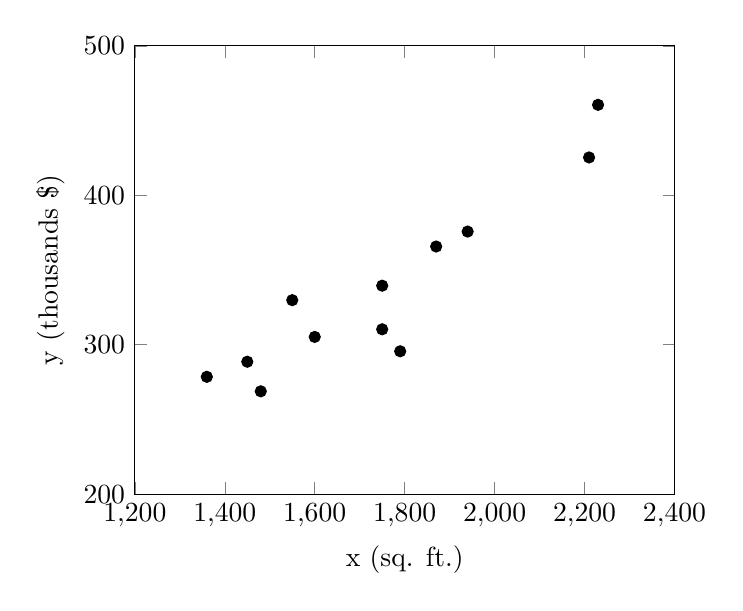
\begin{tikzpicture}
			\begin{axis}[
				xlabel={x (sq. ft.)},
				ylabel={y (thousands \$)},
				xmin=1200, xmax=2400,
				ymin=200, ymax=500,
				]
				\addplot[only marks] coordinates {(1360,278.5) (1940,375.7) (1750,339.5) (1550,329.8) (1790,295.6) (1750,310.3) (2230,460.5) (1600,305.2) (1450,288.6) (1870,365.7) (2210,425.3) (1480,268.8)};
			\end{axis}
		\end{tikzpicture}
	\end{example}
	\subsection{The Least-Squares Line}
	Best-fitting line for linear patterns: $  \hat{y} = a + b x  $
	\begin{definition}[Slope and Intercept]
		$   b = r \left( \frac{s_y}{s_x} \right), \quad a = \bar{y} - b \bar{x}   $
	\end{definition}
	Detailed Explanation: Minimizes squared vertical distances from points to line. Use for prediction when x is independent. b indicates change in y per unit x; a is y when x=0.
	\begin{example}[Work Experience and Wage]
		Data: x (years), y (wage \$):
		$  \bar{x} = 4.5  $, $  \bar{y} = 12.333  $, $  s_x = 1.871  $, $  s_y = 3.710  $, r = 0.980
		$   b = 0.980 \times \frac{3.710}{1.871} \approx 1.943, \quad a = 12.333 - 1.943 \times 4.5 \approx 3.590   $
		Line: $  \hat{y} = 3.590 + 1.943 x  $
		Predict for x=3: $  \hat{y} \approx 9.419  $
		\begin{tikzpicture}
			\begin{axis}[
				xlabel={x (Years)},
				ylabel={y (Wage \$)},
				xmin=0, xmax=8,
				ymin=0, ymax=20,
				]
				\addplot[only marks] coordinates {(2,8) (3,9.5) (4,10) (5,14) (6,15) (7,17.5)};
				\addplot[domain=0:8] {3.59 + 1.943*x};
			\end{axis}
		\end{tikzpicture}
	\end{example}
	\section{Chapter Review}
	For bivariate data: Use contingency tables and comparative charts for categorical; scatterplots, correlation r (-1 to 1), and least-squares line $  \hat{y} = a + b x  $ for quantitative. Identify patterns, strength, direction, outliers.
\end{document}